\chapter{Построение фундаментальной диаграммы \(Q(\rho)\)}\label{ch:ch2}

Фундаментальная диаграмма потока~--- одно из ключевых понятий главы~\ref{ch:ch1} задает функцональную зависимость величины потока (а значит и скорости) АТС от их плотности.
Однако, её расчёт может быть не только лишь чисто теоретическим, но и основанным на реально наблюдаемых данных.
В данной работе для вычислений нам необходимо получить из экспериментальных данных функциональную зависимость \(Q(\rho)\) для всех участков моделируемой автомагистрали.
Для этого предлагается следующий алгоритм использующий данные с дорожных датчиков для восстановления фундаментальной диаграммы на любом сегменте транспортной сети.
Более полно результаты данной работы, полученной группой исследователей, описаны в статье~\cite{collectiveArticle2}.

Построение фундаментальной диаграммы на реальных данных, как правило, весьма трудоёмко, так как практически нет универсальных алгоритмов, автоматически обрабатывающих данные, которые необходимы для выполнения данной задачи. 
Например, широко используемый метод линейной регрессии (см., например,~\cite{wang2011logistic}) недостаточно интерполирует данные в заторных областях из-за малого количества наблюдений в них. 
Именно поэтому так важно создать такой алгоритм, поскольку обрабатывать данные вручную при том, что на сегодняшний день в одной только Москве установлено более 3000 детекторов транспорта, являющихся основным источником данных для данной работы, не представляется возможным.

Данные измерений с автострадных датчиков, а также данные с GPS-треков, позволяют идентифицировать фундаментальные диаграммы для соответствующих участков автострады. Дадим описание алгоритма калибровки:
\begin{enumerate}
  \item Для каждого участка автомагистрали извлечём данные измерений плотности и потока за наблюдаемый период времени. 
        Каждая точка на диаграмме определяется парой значений плотность-поток, на плоскости. (см. например рис.~\ref{fig:detectors_data_alpha})
  \item Фильтруем данные, отбрасывая экстремальные значения с использованием алгоритма построения альфа-оболочек. 
        Сначала, мы масштабируем данные вдоль осей \(Q\) и \(\rho\), чтобы получить одинаковые порядки величин. 
        Затем, по результирующем точкам мы строим альфа-оболочку~\cite{edelsbrunner1983shape}, и удаляем точки, попавшие на оболочку~\cite{eddy19825th}. 
        Процесс повторяется до тех пор, пока разница в площади оболочек между соседними итерациями составит менее 5\%, либо пока не останется менее 90\% начальных точек. (рис.~\ref{fig:detectors_data_alpha}, нижние графики)
  \item Среди измерений найдём максимальный поток \(Q_1(\rho_1) = \max_{\rho}[Q(\rho)]\) и его плотность \(\rho_1\), которая является критической, поскольку при её прохождении обычно интенсивность транспортного потока заметно падает.
  \item Находим максимальное значение интенсивности \(Q_0(\rho_0) = \max_{Q}[Q(\rho_1 / 2)]\) для значения плотности \(\rho_0 = \rho_1 / 2\)
  \item Далее среди измерений найдём максимально удалённую точку от начала координат на плоскости  \(Q(\rho):\ \max \sqrt{(Q/Q_{max})^2 + (\rho/\rho_{max})^2}\).
  \item Используя знания геометрии дороги, определим максимально возможную плотность \(\rho_*\), как произведение количества линий на дороге на значение 0.15 АТС/м, исходя из известной оценки, что при количестве АТС больше 150 на один километр движение транспорта становится невозможным.
  \item Далее переходим к получению функциональной зависимости интенсивности транс-портного потока от его плотности \(Q(\rho)\)
\end{enumerate}
\begin{figure}[ht]
\begin{center}
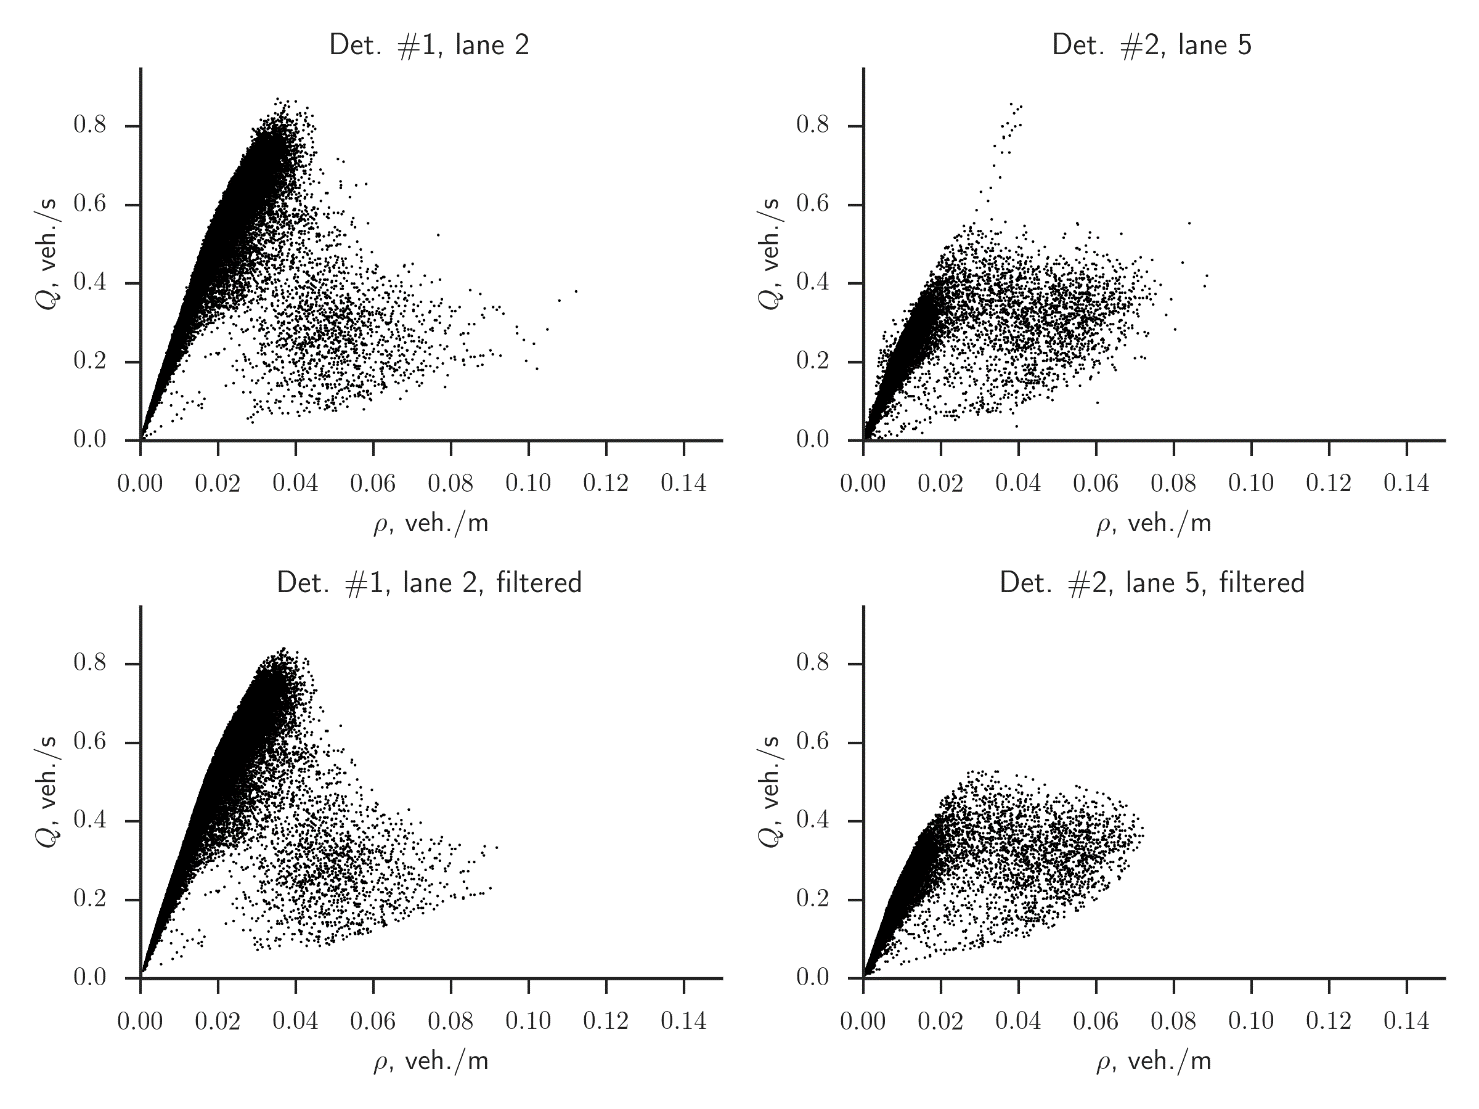
\includegraphics[width=1\linewidth]{detectors_data_alpha.png}
\caption{Экспериментальные данные с двух детекторов, установленных на различных полосах МКАД --- замеренные интенсивности транспортного потока \(Q(\rho)\)[АТС/с] при различной плотности [АТС/м]. Данные представлены за 2012 г. В количестве 288 измерений за день. Сверху исходные данные, снизу отфильтрованные с использованием алгоритма построения выпуклых оболочек.}
\label{fig:detectors_data_alpha}
\end{center}
\end{figure}
В соответствии с теорией трёх фаз транспортного потока Б.С. Кернера на скоростных автомагистралях~\cite{kerner2009introduction} кратко изложенной в разделе~\cref{subsec:ch1/sec4_kerner} выделяем три фазы транспортного потока:
\begin{enumerate}
  \item Свободный поток \(Q(0\leq\rho\leq\rho_1)\)
  \item Синхронизованный поток \(Q(\rho_1\leq\rho\leq\rho_2)\)
  \item Заторный поток \(Q(\rho_1\leq\rho\leq\rho_*)\)
\end{enumerate}
Для каждой из фаз транспортного потока задаём её собственную функциональную зависимость \(Q(\rho)\), сшивая их в точках фазового перехода:
\begin{enumerate}
  \item Свободный поток \(Q(\rho) = \alpha_2\rho^2 + \alpha_1\rho,\ 0\leq\rho\leq\rho_1\)
  \item Синхронизованный поток \(Q(\rho) = \beta_2\rho^2 + \beta_1\rho + \beta_0,\ \rho_1\leq\rho\leq\rho_2\)
  \item Заторный поток \(Q(\rho) = c_*(\rho_*-\rho),\ \rho_1\leq\rho\leq\rho_*\)
\end{enumerate}
Коэффициенты функциональных зависимостей находим, приравнивая значения функций в найденных точках к значениям интенсивностей в них, в результате получаем следующую систему уравнений:
\begin{displaymath}\left\{
\begin{array}{llllll}
  \alpha_2\rho_0^2 + \alpha_1\rho_0 = Q(\rho_0)\\
  \alpha_2\rho_1^2 + \alpha_1\rho_1 = Q(\rho_1)\\
  \beta_2\rho_1^2 + \beta_1\rho_1 + \beta_0 = Q(\rho_1)\\
  \beta_2\rho_2^2 + \beta_1\rho_2 + \beta_0 = Q(\rho_2)\\
  2\beta_2\rho_1 + \beta_1 = c_1 = \left.\frac{\partial Q(\rho)}{\partial \rho}\right|_{\rho = \rho_1}\\
  c_*(\rho_*-\rho_2) = Q(\rho_2)
\end{array} \right.
\end{displaymath}
Осталось только понять чему будет равна производная функции после прохождения критической точки: $\left.\frac{\partial Q(\rho)}{\partial \rho}\right|_{\rho = \rho_1} = c_1 = ?$.
Из экспериментальных наблюдений мы знаем, что после её прохождения интенсивность транспортного потока заметно падает. Это означает, что поток начинает тормозиться, поэтому логично предположить, что $c_1$ есть скорость волны торможения и её можно найти, построив пространственно-временную структуру или карту значений скорости транспортного потока для соответствующих участков автострады (см рис.~\ref{fig:cstart}).

Отметим, что для построения пространственно-временной структуры транспортного потока зачастую недостаточно одних лишь дорожных датчиков, так как они расположены по автомагистрали с недостаточной плотностью.
Тут важную роль играют GPS-треки.
Их ключевой недостаток заключается в том, что GPS фиксирует движение только некоторой доли автомобилей из общего потока.
Доля эта может меняться как в зависимости от фазы потока (плотности движения АТС) так и от времени суток.
Характеристики этой зависимости зачастую связаны с характером источника данных.
Так, например, службы такси будут иметь лучшее покрытие в то время, когда число заказов наибольшее.
Однако, этот недостаток никак не влияет на измеряемую с помощью GPS-треков скорость автомобилей, что позволяет без каких либо ограничений использовать эти данные для построения фундаментальной диаграммы.
\begin{figure}[ht]
\begin{center}
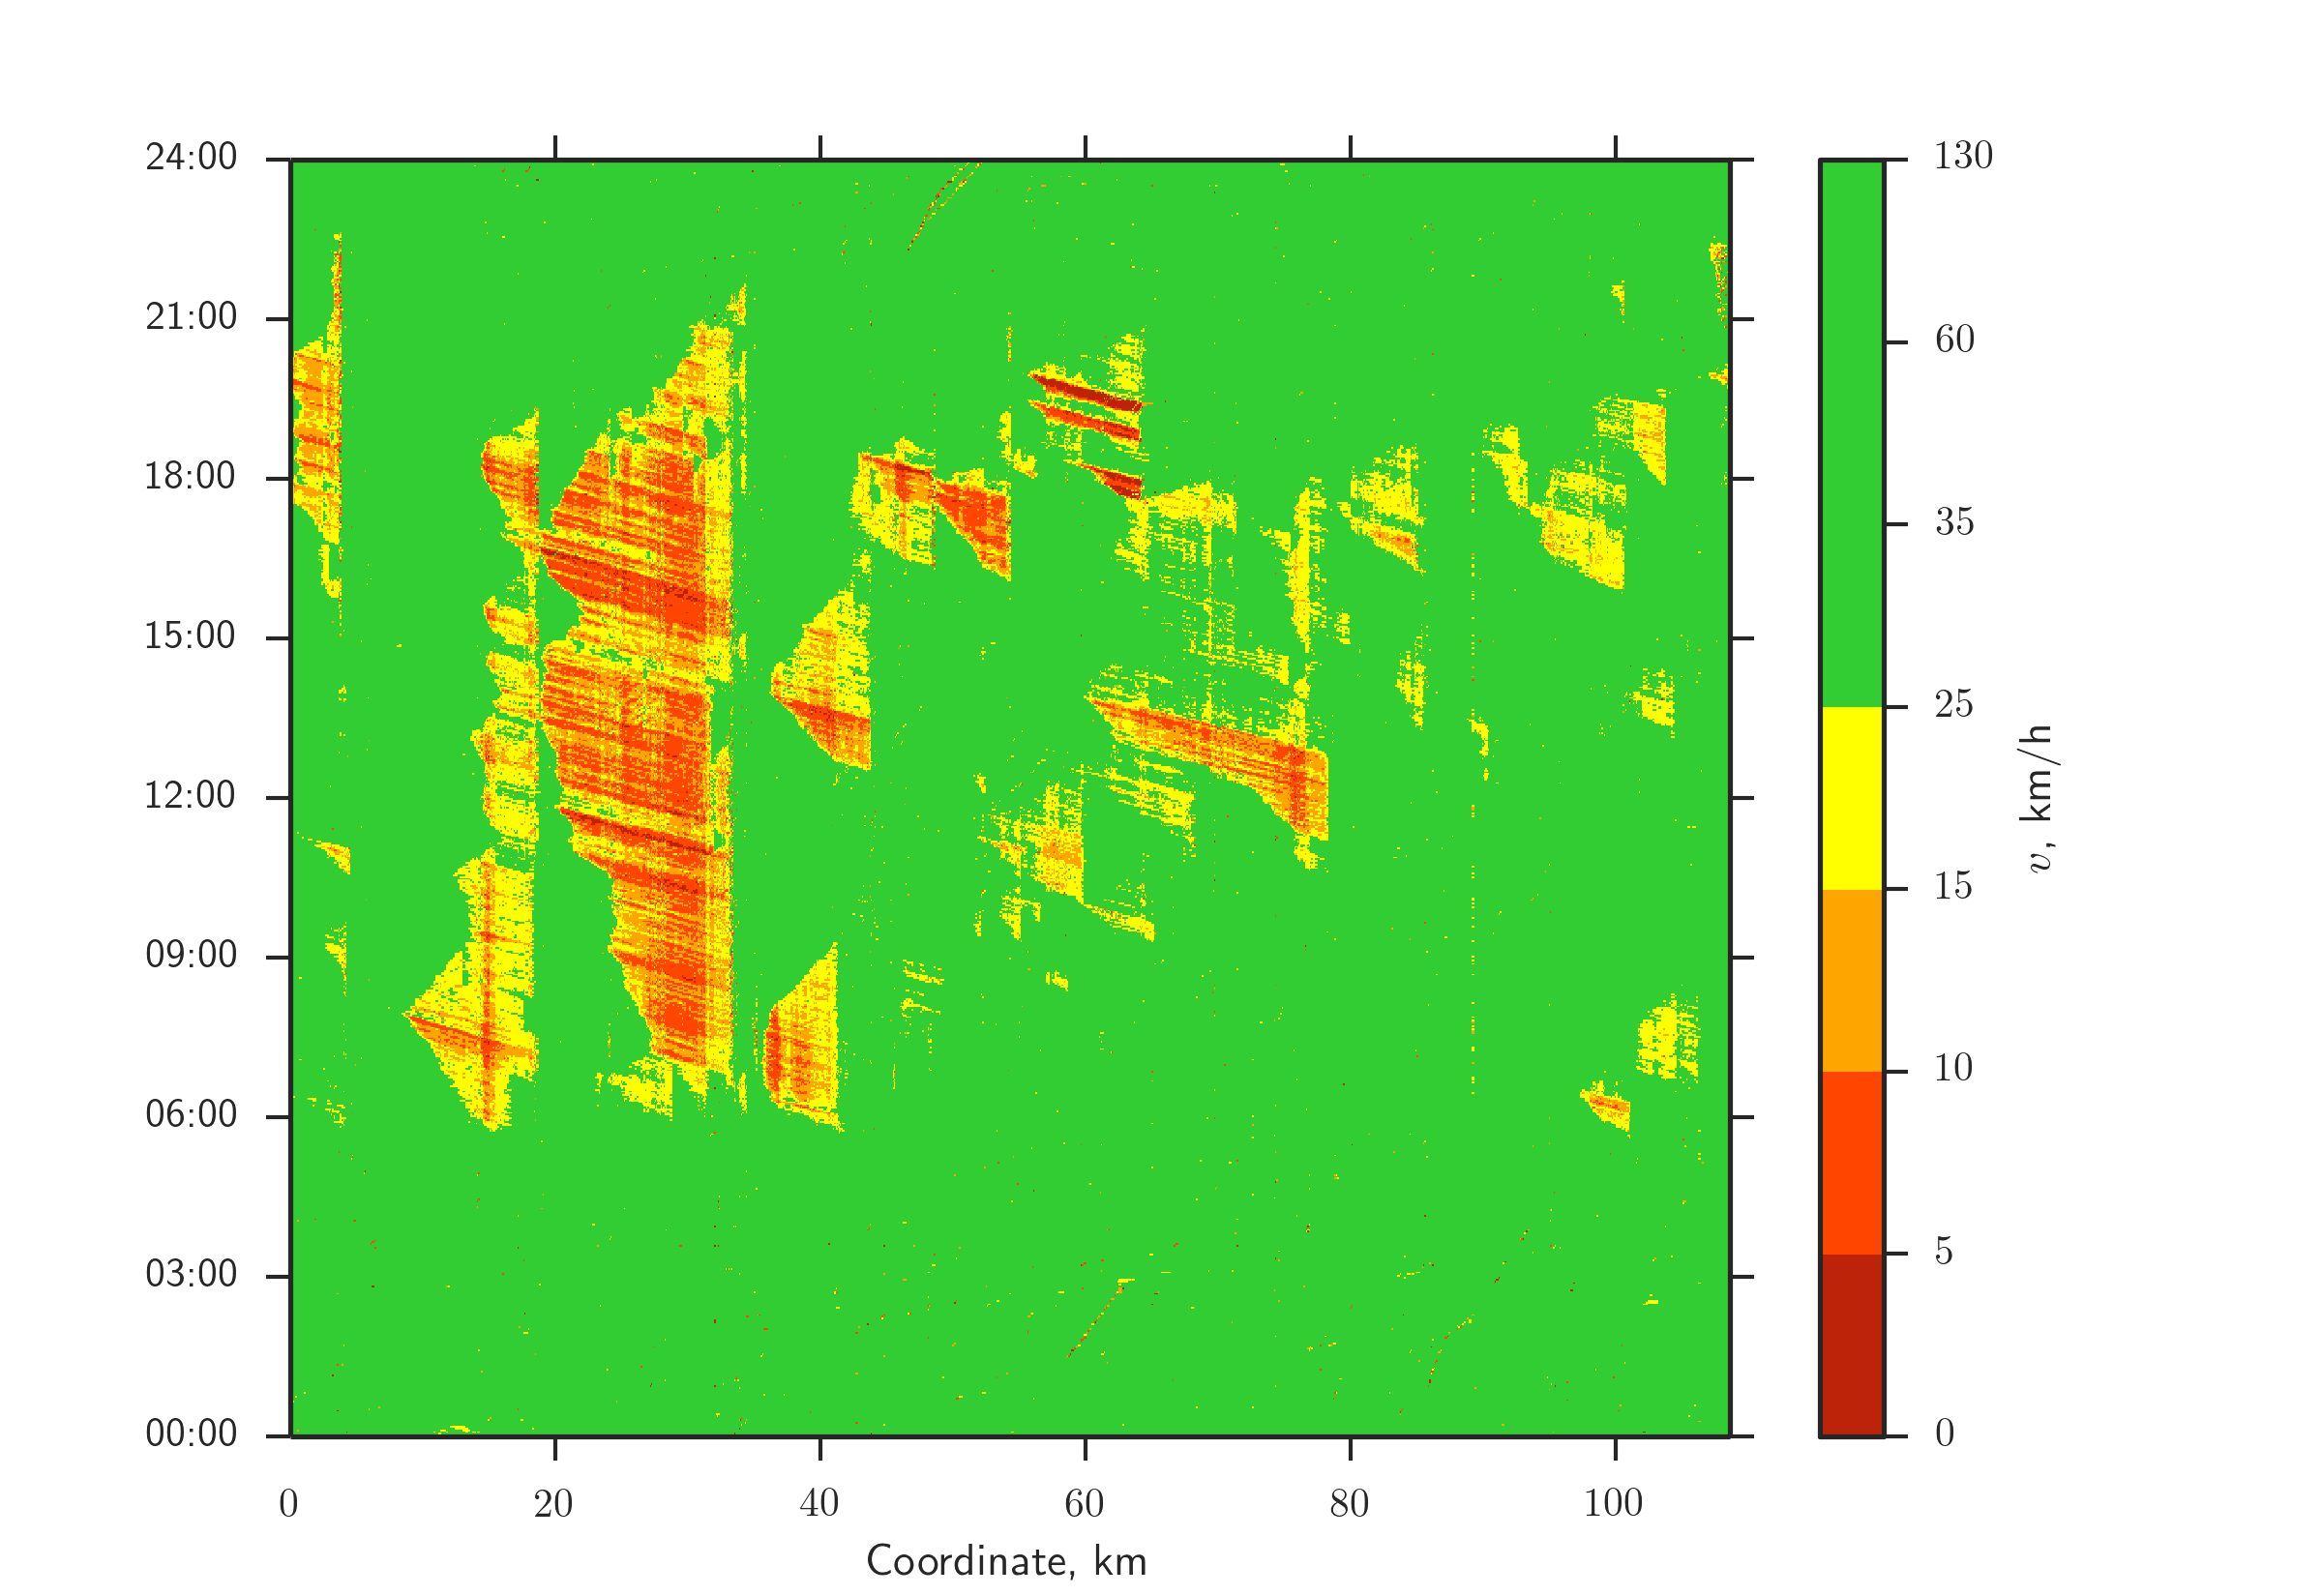
\includegraphics[width=1\linewidth]{c_start.png}
\caption{Пространственно-временная структура значений скорости транспортного потока на внешней стороне МКАД для одного рабочего дня --- 5 декабря 2012 г.}
\label{fig:cstart}
\end{center}
\end{figure}


На рисунке~\ref{fig:cstart} хорошо видны красные линии распространения волн торможения навстречу движению транспортного потока. 
Наклон этих линий, которые со временем остаются параллельными, и есть значение скорости волны торможения. 
Следующая проблема, которую предстоит решить, это как автоматизировать процесс нахождения значений скорости волн торможения по карте скоростей для заданного участка дороги. 
Эта задача была решена с использованием алгоритмов компьютерного зрения~\cite{bradski2000dr} в три этапа~\ref{fig:cend}:
\begin{enumerate}
  \item Выделение границ методом Кэнни~\cite{canny1986computational} --- рис.~\ref{fig:cend}(cлева)
  \item Поиск отрезков среди выделенных границ методом Хафа~\cite{matas2000robust}  --- рис.~\ref{fig:cend}(центр)
  \item Отсеивание ложных линий  --- рис.~\ref{fig:cend}(cправа)
\end{enumerate}
\begin{figure}[ht]
\begin{center}
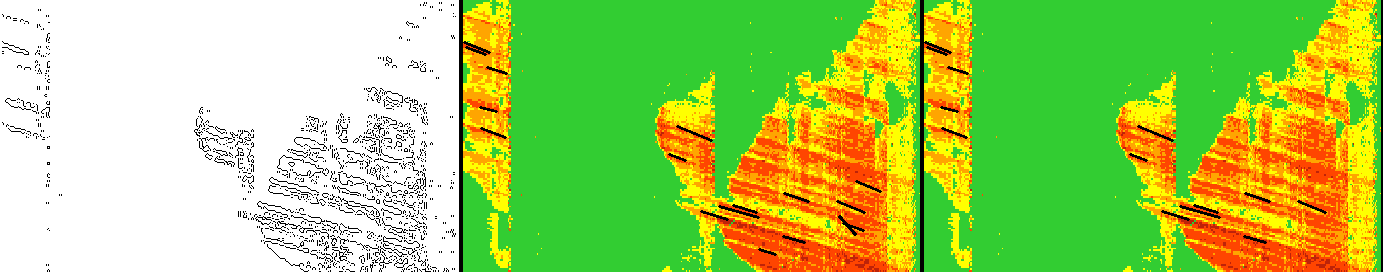
\includegraphics[width=1\linewidth]{c_end.png}
\caption{Нахождение значений скорости волн торможения на пространственно-временной структуре значений скорости транспортного потока на внешней стороне МКАД}
\label{fig:cend}
\end{center}
\end{figure}


Как результат этой работы, была получена гистограмма значений скоростей волны торможения транспортного потока на внешней стороне МКАД~\ref{fig:chist} за 2012 г.

\begin{figure}[ht]
\begin{center}
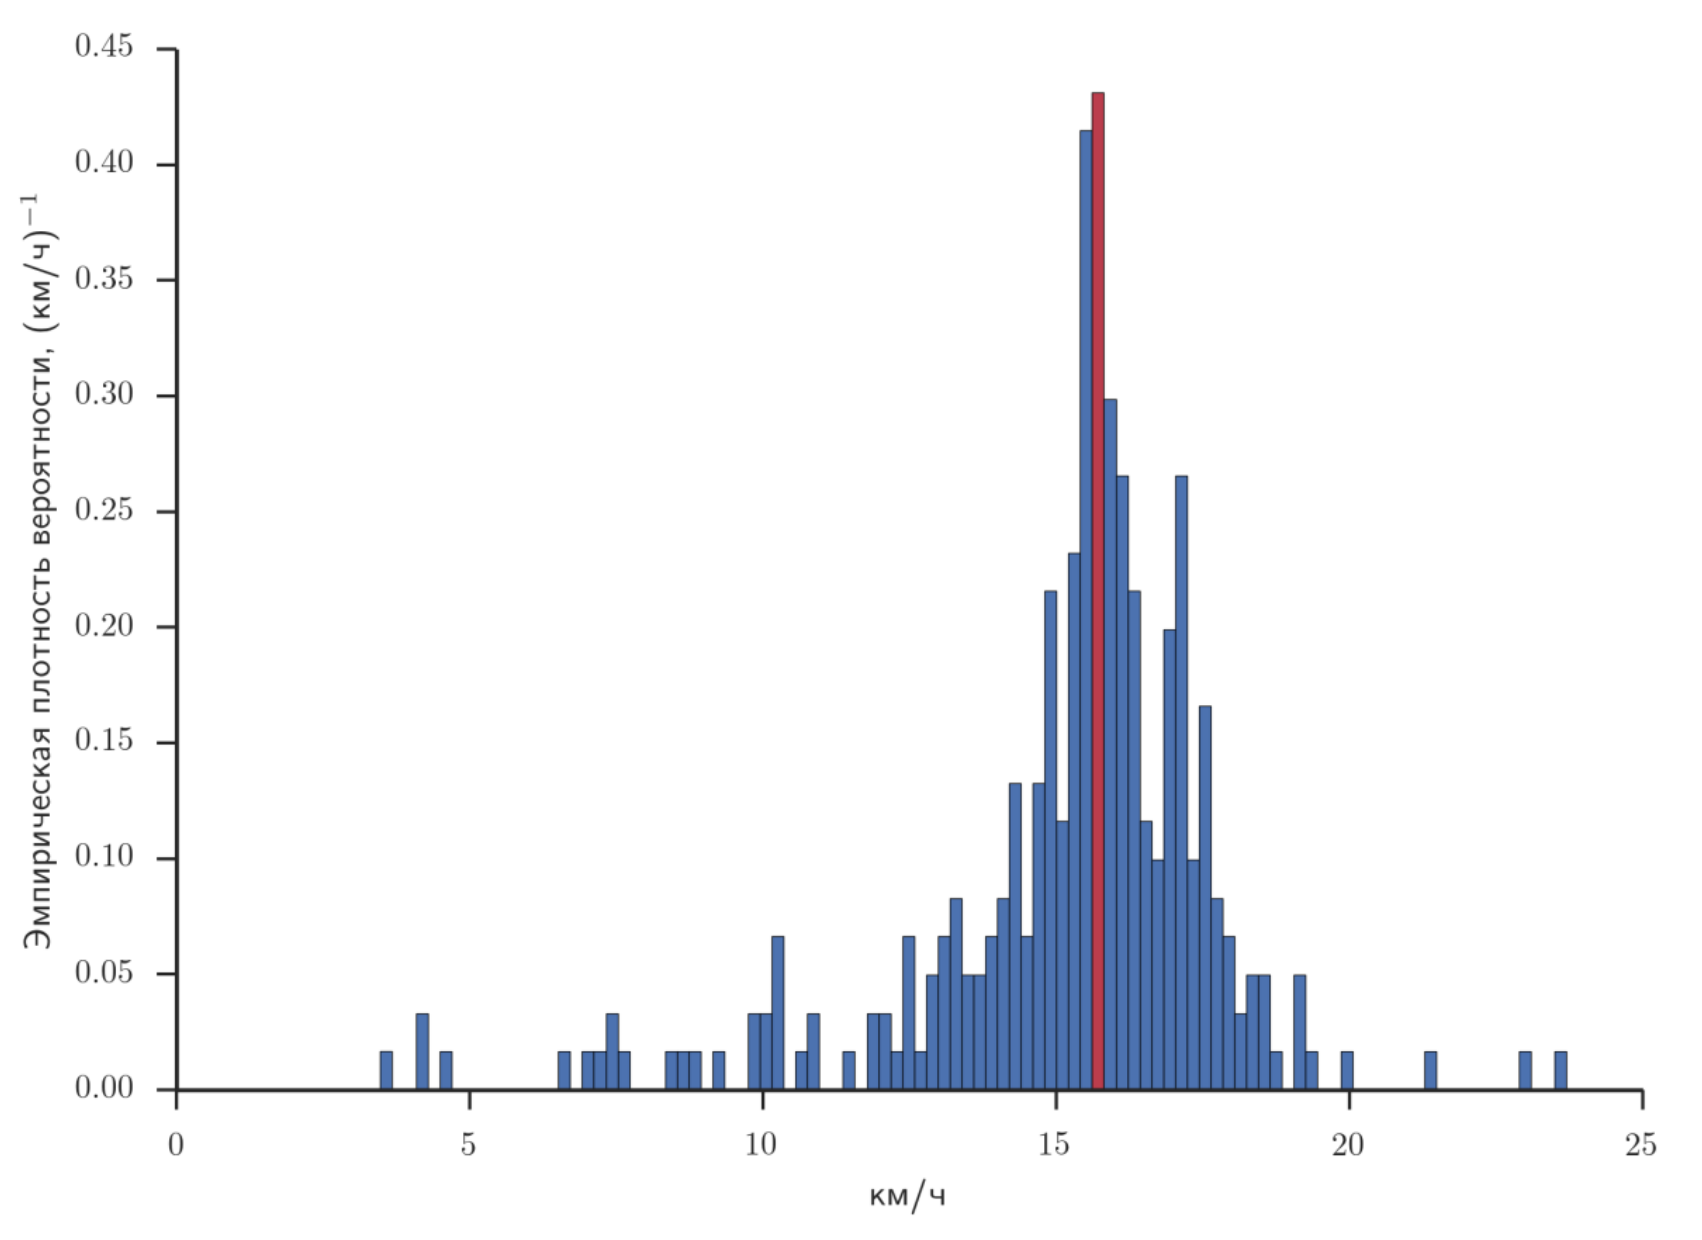
\includegraphics[width=0.9\linewidth]{chist_speed_wave.png}
\caption{Гистограмма значений скоростей волны торможения транспортного потока на МКАД за 2012 г}
\label{fig:chist}
\end{center}
\end{figure}
Отсеяв ложные значения, мы установили, что скорость волны торможения на МКАД \(\left.\frac{\partial Q(\rho)}{\partial \rho}\right|_{\rho = \rho_1} = c_1 = -15.8\) [км/ч], также мы выяснили, что она не зависит от времени года, дня недели и определяется исключительно геометрией дороги.
Данная скорость очень близка к скорости приводимой Кернером~\cite{kerner2009introduction} как скорость <<заднего фронта широко движущегося кластера>>: \(v_g \approx -15\) [км/ч].
Таким образом, в отсутствии достаточно объёмных данных о скорости движения АТС, к чему зачастую ведет отсутствие данных с GPS-треков, можно использовать скорость в -15 [км/ч].

Полученные в итоге примеры фундаментальных диаграмм представлены на рис.~\ref{fig:qresult}
\begin{figure}[ht]
\begin{center}
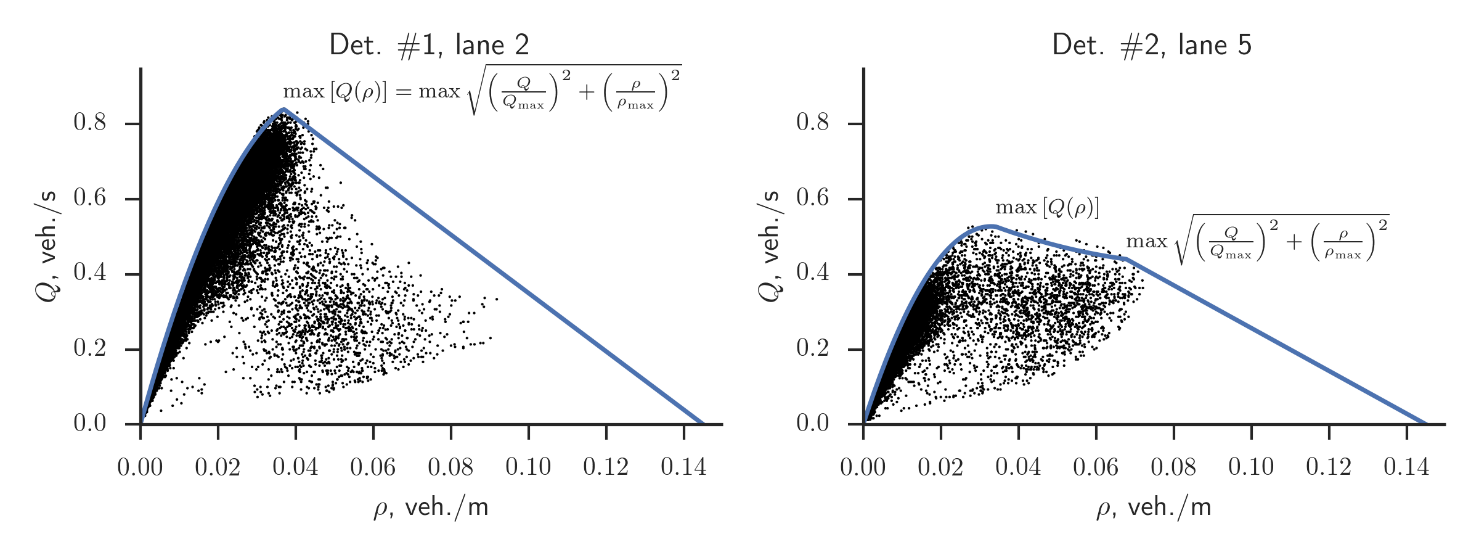
\includegraphics[width=1\linewidth]{Q_result.png}
\caption{Фундаментальные диаграммы для двух разных участков МКАД. Слева для данных со второй полосы (детектор № 1), справа с пятой полосы (детектор №2)}
\label{fig:qresult}
\end{center}
\end{figure}

\FloatBarrier
